\subsection{Experiment One: Best Input Combination}

\subsubsection{Best Input Combination Results}
\label{sec:simpleInputTest}
The simple input test based on 3 month historical data and 200 epochs.

WS = Wind Speed
AD = Air Density
C = Consumption
T = Temperature
WD = Wind Direction
L-P = Last Known Production
D = Date
ToD = Time of Day
M = Time of Day as matrix
CD = Correct Direction

\footnotesize
\begin{center}
\begin{longtable}{|c|c|c|c|c|c|c|c|c|c|c|c|c|}
\caption{Wind Production Input Parameter Test}\\
\hline
\textbf{WS} & \textbf{AD} & \textbf{C} & \textbf{T} & \textbf{WD} & \textbf{L-P} & \textbf{D}& \textbf{ToD} & \textbf{MAE} & \textbf{\% from \#1} & \textbf{H1} & \textbf{H2} & \textbf{CD} \\
\hline
\endfirsthead
\multicolumn{13}{c}%
{\tablename\ \thetable\ -- \textit{Continued from previous page}} \\
\hline
\textbf{WS} & \textbf{AD} & \textbf{C} & \textbf{T} & \textbf{WD} & \textbf{L-P} & \textbf{D}& \textbf{ToD} & \textbf{MAE} & \textbf{\% from \#1} & \textbf{H1} & \textbf{H2} & \textbf{CD}  \\
\hline
\endhead
\hline \multicolumn{13}{r}{\textit{Continued on next page}} \\
\endfoot
\hline
\endlastfoot
\arrayrulecolor{light-gray}
 \x &  &  &  \x &  &  \x &  &  \x & 128,32 & 0,0\% & 24 & 1 & 73\% \\ \hline
 \x &  \x &  &  &  \x &  \x &  &  \x & 131,59 & 2,55\% & 17 & 1 & 73\% \\ \hline
 \x &  \x &  &  &  &  \x &  &  \x & 131,89 & 2,78\% & 12 & 1 & 73\% \\ \hline
 \x &  \x &  \x &  \x &  \x &  \x &  &  \x & 133,18 & 3,79\% & 22 & 1 & 72\% \\ \hline
 \x &  \x &  \x &  \x &  \x &  \x &  &  & 133,77 & 4,25\% & 24 & 1 & 73\% \\ \hline
 \x &  \x &  \x &  &  &  \x &  &  \x & 134,14 & 4,54\% & 19 & 1 & 73\% \\ \hline
 \x &  \x &  \x &  &  \x &  \x &  &  \x & 135,4 & 5,52\% & 25 & 1 & 72\% \\ \hline
 \x &  \x &  \x &  &  &  \x &  &  & 136,33 & 6,24\% & 15 & 1 & 73\% \\ \hline
 \x &  \x &  &  &  &  \x &  \x &  \x & 136,65 & 6,49\% & 11 & 1 & 73\% \\ \hline
 \x &  &  &  &  &  \x &  &  & 137,33 & 7,02\% & 1 & 0 & 74\% \\ \hline
 \x &  &  &  \x &  \x &  \x &  &  \x & 137,8 & 7,39\% & 10 & 1 & 73\% \\ \hline
 \x &  \x &  &  &  \x &  \x &  &  & 138,16 & 7,67\% & 17 & 1 & 72\% \\ \hline
 \x &  &  \x &  &  &  &  &  & 138,33 & 7,8\% & 11 & 1 & 64\% \\ \hline
 \x &  \x &  &  \x &  &  \x &  &  & 138,94 & 8,28\% & 20 & 1 & 72\% \\ \hline
 \x &  \x &  &  &  &  &  &  \x & 139,25 & 8,52\% & 24 & 1 & 54\% \\ \hline
 \x &  \x &  &  &  &  \x &  &  & 139,35 & 8,6\% & 24 & 1 & 73\% \\ \hline
 \x &  \x &  \x &  &  &  &  &  & 139,67 & 8,85\% & 17 & 1 & 64\% \\ \hline
 \x &  &  \x &  &  \x &  \x &  &  \x & 139,78 & 8,93\% & 18 & 1 & 71\% \\ \hline
 \x &  \x &  \x &  \x &  &  &  &  & 139,99 & 9,09\% & 21 & 1 & 64\% \\ \hline
 \x &  &  &  &  &  &  &  \x & 140,14 & 9,21\% & 14 & 1 & 41\% \\ \hline
 \x &  &  &  &  \x &  &  &  \x & 140,44 & 9,45\% & 25 & 1 & 61\% \\ \hline
 \x &  &  &  \x &  &  \x &  &  & 140,55 & 9,53\% & 24 & 1 & 73\% \\ \hline
 \x &  &  \x &  &  &  \x &  &  & 140,82 & 9,74\% & 18 & 1 & 73\% \\ \hline
 \x &  \x &  \x &  &  &  &  &  \x & 140,85 & 9,76\% & 23 & 1 & 64\% \\ \hline
 \x &  \x &  \x &  \x &  &  \x &  &  \x & 140,91 & 9,81\% & 14 & 1 & 73\% \\ \hline
 \x &  \x &  &  &  &  &  &  & 141,09 & 9,95\% & 7 & 1 & 53\% \\ \hline
 \x &  &  \x &  &  &  &  &  \x & 141,28 & 10,1\% & 11 & 1 & 64\% \\ \hline
 \x &  &  \x &  &  \x &  &  &  \x & 141,38 & 10,18\% & 18 & 1 & 65\% \\ \hline
 \x &  &  &  &  \x &  &  &  & 141,5 & 10,27\% & 16 & 1 & 60\% \\ \hline
 \x &  &  &  &  \x &  \x &  &  & 142,22 & 10,83\% & 24 & 1 & 72\% \\ \hline
 \x &  \x &  \x &  \x &  &  \x &  \x &  \x & 142,35 & 10,93\% & 13 & 1 & 72\% \\ \hline
 \x &  \x &  &  \x &  \x &  &  &  \x & 142,44 & 11,0\% & 20 & 1 & 61\% \\ \hline
 \x &  \x &  \x &  &  &  \x &  \x &  \x & 142,57 & 11,11\% & 20 & 1 & 73\% \\ \hline
 \x &  \x &  &  \x &  &  \x &  &  \x & 142,64 & 11,16\% & 17 & 1 & 72\% \\ \hline
 \x &  &  \x &  &  &  \x &  &  \x & 142,67 & 11,18\% & 14 & 1 & 72\% \\ \hline
 \x &  \x &  \x &  &  \x &  &  &  & 142,75 & 11,25\% & 15 & 1 & 63\% \\ \hline
 \x &  &  \x &  \x &  \x &  \x &  &  \x & 142,97 & 11,42\% & 15 & 1 & 71\% \\ \hline
 \x &  \x &  &  &  \x &  &  &  \x & 143,07 & 11,49\% & 20 & 1 & 61\% \\ \hline
 \x &  \x &  \x &  &  &  &  \x &  \x & 143,23 & 11,62\% & 20 & 1 & 64\% \\ \hline
 \x &  &  \x &  \x &  &  \x &  &  \x & 143,24 & 11,63\% & 15 & 1 & 72\% \\ \hline
 \x &  \x &  &  \x &  &  &  &  \x & 143,53 & 11,85\% & 24 & 1 & 54\% \\ \hline
 \x &  \x &  &  &  \x &  &  &  & 143,98 & 12,2\% & 19 & 1 & 61\% \\ \hline
 \x &  \x &  \x &  &  \x &  &  &  \x & 144,06 & 12,27\% & 11 & 1 & 63\% \\ \hline
 \x &  \x &  \x &  &  &  \x &  \x &  & 144,24 & 12,41\% & 13 & 1 & 71\% \\ \hline
 \x &  &  &  \x &  \x &  \x &  &  & 144,95 & 12,96\% & 10 & 1 & 72\% \\ \hline
 \x &  \x &  \x &  &  \x &  \x &  &  & 144,96 & 12,97\% & 17 & 1 & 71\% \\ \hline
 \x &  &  &  &  &  \x &  &  \x & 145,11 & 13,08\% & 20 & 1 & 72\% \\ \hline
 \x &  \x &  &  \x &  \x &  \x &  &  & 145,26 & 13,2\% & 12 & 1 & 72\% \\ \hline
 \x &  \x &  \x &  \x &  &  &  &  \x & 145,49 & 13,38\% & 8 & 1 & 65\% \\ \hline
 \x &  &  \x &  &  \x &  \x &  \x &  & 145,92 & 13,72\% & 20 & 1 & 73\% \\ \hline
 \x &  &  \x &  &  \x &  &  \x &  \x & 145,98 & 13,76\% & 25 & 1 & 64\% \\ \hline
 \x &  &  \x &  &  &  &  \x &  \x & 146,02 & 13,79\% & 10 & 1 & 64\% \\ \hline
 \x &  \x &  \x &  \x &  &  &  \x &  \x & 146,32 & 14,03\% & 17 & 1 & 64\% \\ \hline
 \x &  &  \x &  \x &  &  &  &  \x & 146,48 & 14,15\% & 10 & 1 & 64\% \\ \hline
 \x &  &  \x &  &  \x &  &  &  & 146,82 & 14,42\% & 21 & 1 & 64\% \\ \hline
 \x &  \x &  &  &  &  &  \x &  \x & 147,08 & 14,62\% & 17 & 1 & 54\% \\ \hline
 \x &  &  &  \x &  &  &  &  & 147,41 & 14,88\% & 1 & 0 & 51\% \\ \hline
 \x &  \x &  &  \x &  \x &  \x &  \x &  \x & 147,99 & 15,33\% & 12 & 1 & 72\% \\ \hline
 \x &  \x &  \x &  \x &  &  \x &  \x &  & 148,27 & 15,55\% & 13 & 1 & 72\% \\ \hline
 \x &  &  \x &  \x &  \x &  \x &  &  & 148,61 & 15,81\% & 13 & 1 & 71\% \\ \hline
 \x &  &  &  \x &  \x &  &  &  \x & 148,67 & 15,86\% & 24 & 1 & 60\% \\ \hline
 \x &  &  &  \x &  &  &  &  \x & 149,27 & 16,33\% & 25 & 1 & 51\% \\ \hline
 \x &  &  &  &  &  &  &  & 149,72 & 16,68\% & 20 & 1 & 41\% \\ \hline
 \x &  &  \x &  &  &  &  \x &  & 149,8 & 16,74\% & 15 & 1 & 64\% \\ \hline
 \x &  \x &  \x &  \x &  &  \x &  &  & 149,85 & 16,78\% & 21 & 1 & 71\% \\ \hline
 \x &  &  &  &  &  \x &  \x &  \x & 150,3 & 17,13\% & 11 & 1 & 72\% \\ \hline
 \x &  \x &  \x &  \x &  &  &  \x &  & 150,45 & 17,25\% & 20 & 1 & 64\% \\ \hline
 \x &  &  \x &  \x &  \x &  &  &  & 150,63 & 17,39\% & 22 & 1 & 63\% \\ \hline
 \x &  &  \x &  \x &  &  \x &  &  & 150,96 & 17,64\% & 17 & 1 & 71\% \\ \hline
 \x &  &  \x &  &  \x &  \x &  &  & 151,54 & 18,1\% & 21 & 1 & 71\% \\ \hline
 \x &  &  &  &  \x &  \x &  &  \x & 151,55 & 18,1\% & 19 & 1 & 72\% \\ \hline
 \x &  &  \x &  &  &  \x &  \x &  \x & 151,92 & 18,39\% & 8 & 1 & 72\% \\ \hline
 \x &  \x &  &  &  \x &  \x &  \x &  & 152,61 & 18,93\% & 17 & 1 & 71\% \\ \hline
 \x &  \x &  \x &  &  \x &  &  \x &  & 152,89 & 19,15\% & 16 & 1 & 63\% \\ \hline
 \x &  \x &  &  &  &  &  \x &  & 153,3 & 19,47\% & 21 & 1 & 54\% \\ \hline
 \x &  \x &  &  &  \x &  &  \x &  & 153,31 & 19,47\% & 16 & 1 & 61\% \\ \hline
 \x &  &  &  &  &  &  \x &  & 153,92 & 19,95\% & 12 & 1 & 41\% \\ \hline
 \x &  &  \x &  \x &  &  &  &  & 154,02 & 20,03\% & 14 & 1 & 63\% \\ \hline
 \x &  \x &  \x &  \x &  \x &  &  &  \x & 154,25 & 20,21\% & 15 & 1 & 63\% \\ \hline
 \x &  \x &  \x &  &  \x &  &  \x &  \x & 154,51 & 20,41\% & 12 & 1 & 64\% \\ \hline
 \x &  &  &  &  \x &  &  \x &  & 154,58 & 20,46\% & 17 & 1 & 59\% \\ \hline
 \x &  \x &  &  &  &  \x &  \x &  & 154,85 & 20,67\% & 13 & 1 & 72\% \\ \hline
 \x &  \x &  &  \x &  &  &  \x &  & 154,97 & 20,77\% & 20 & 1 & 54\% \\ \hline
 \x &  \x &  &  \x &  \x &  &  \x &  \x & 155,07 & 20,85\% & 22 & 1 & 61\% \\ \hline
 \x &  \x &  &  \x &  &  &  \x &  \x & 155,55 & 21,22\% & 14 & 1 & 54\% \\ \hline
 \x &  &  &  &  \x &  &  \x &  \x & 156,13 & 21,67\% & 18 & 1 & 60\% \\ \hline
 \x &  \x &  \x &  \x &  \x &  &  &  & 156,26 & 21,77\% & 12 & 1 & 62\% \\ \hline
 \x &  &  \x &  \x &  &  &  \x &  \x & 156,52 & 21,98\% & 15 & 1 & 64\% \\ \hline
 \x &  &  \x &  \x &  \x &  &  \x &  & 156,72 & 22,13\% & 17 & 1 & 63\% \\ \hline
 \x &  \x &  &  \x &  \x &  &  &  & 156,94 & 22,3\% & 13 & 1 & 60\% \\ \hline
 \x &  &  \x &  &  &  \x &  \x &  & 157,19 & 22,5\% & 19 & 1 & 72\% \\ \hline
 \x &  &  &  &  &  &  \x &  \x & 157,36 & 22,63\% & 15 & 1 & 40\% \\ \hline
 \x &  &  \x &  \x &  \x &  &  &  \x & 157,44 & 22,69\% & 17 & 1 & 62\% \\ \hline
 \x &  \x &  &  &  \x &  &  \x &  \x & 157,56 & 22,79\% & 19 & 1 & 60\% \\ \hline
 \x &  \x &  \x &  &  &  &  \x &  & 157,71 & 22,9\% & 14 & 1 & 61\% \\ \hline
 \x &  &  &  \x &  \x &  &  \x &  & 158,06 & 23,18\% & 22 & 1 & 60\% \\ \hline
 \x &  \x &  &  \x &  &  &  &  & 158,3 & 23,36\% & 13 & 1 & 50\% \\ \hline
 \x &  &  &  \x &  &  &  \x &  \x & 158,4 & 23,44\% & 22 & 1 & 51\% \\ \hline
 \x &  &  &  &  &  \x &  \x &  & 158,51 & 23,53\% & 13 & 1 & 71\% \\ \hline
 \x &  \x &  \x &  \x &  \x &  &  \x &  \x & 159,52 & 24,31\% & 11 & 1 & 62\% \\ \hline
 \x &  &  \x &  \x &  &  &  \x &  & 159,55 & 24,34\% & 16 & 1 & 64\% \\ \hline
 \x &  &  \x &  \x &  \x &  &  \x &  \x & 160,37 & 24,98\% & 24 & 1 & 62\% \\ \hline
 \x &  \x &  &  \x &  \x &  \x &  &  \x & 160,53 & 25,1\% & 21 & 1 & 71\% \\ \hline
 \x &  &  &  &  \x &  \x &  \x &  \x & 160,56 & 25,12\% & 10 & 1 & 71\% \\ \hline
 \x &  \x &  \x &  \x &  \x &  \x &  \x &  & 160,62 & 25,17\% & 15 & 1 & 71\% \\ \hline
 \x &  &  \x &  \x &  \x &  \x &  \x &  & 161,1 & 25,55\% & 13 & 1 & 70\% \\ \hline
 \x &  &  &  \x &  \x &  &  &  & 161,21 & 25,63\% & 15 & 1 & 60\% \\ \hline
 \x &  &  \x &  &  \x &  \x &  \x &  \x & 161,23 & 25,65\% & 16 & 1 & 70\% \\ \hline
 \x &  &  \x &  &  \x &  &  \x &  & 161,32 & 25,72\% & 20 & 1 & 63\% \\ \hline
 \x &  &  &  \x &  \x &  &  \x &  \x & 165,26 & 28,79\% & 23 & 1 & 59\% \\ \hline
 \x &  &  &  \x &  \x &  \x &  \x &  & 166,87 & 30,04\% & 21 & 1 & 71\% \\ \hline
 \x &  &  &  \x &  &  \x &  \x &  & 167,74 & 30,72\% & 20 & 1 & 70\% \\ \hline
 \x &  &  &  \x &  &  &  \x &  & 167,83 & 30,79\% & 14 & 1 & 49\% \\ \hline
 \x &  \x &  &  \x &  \x &  \x &  \x &  & 168,73 & 31,49\% & 12 & 1 & 69\% \\ \hline
 \x &  \x &  &  \x &  \x &  &  \x &  & 168,81 & 31,55\% & 12 & 1 & 60\% \\ \hline
 \x &  \x &  \x &  &  \x &  \x &  \x &  \x & 169,41 & 32,02\% & 19 & 1 & 71\% \\ \hline
 \x &  \x &  \x &  \x &  \x &  &  \x &  & 169,83 & 32,35\% & 21 & 1 & 62\% \\ \hline
 \x &  &  &  \x &  \x &  \x &  \x &  \x & 169,92 & 32,42\% & 21 & 1 & 70\% \\ \hline
 \x &  \x &  &  \x &  &  \x &  \x &  & 170,93 & 33,21\% & 21 & 1 & 71\% \\ \hline
 \x &  &  \x &  \x &  \x &  \x &  \x &  \x & 171,61 & 33,74\% & 23 & 1 & 71\% \\ \hline
 \x &  &  \x &  \x &  &  \x &  \x &  & 172,72 & 34,6\% & 21 & 1 & 71\% \\ \hline
 \x &  &  &  &  \x &  \x &  \x &  & 173,12 & 34,91\% & 17 & 1 & 71\% \\ \hline
 \x &  &  \x &  \x &  &  \x &  \x &  \x & 173,65 & 35,33\% & 12 & 1 & 69\% \\ \hline
 \x &  \x &  \x &  \x &  \x &  \x &  \x &  \x & 174,26 & 35,8\% & 17 & 1 & 68\% \\ \hline
 \x &  \x &  &  \x &  &  \x &  \x &  \x & 174,55 & 36,03\% & 21 & 1 & 71\% \\ \hline
 \x &  &  &  \x &  &  \x &  \x &  \x & 174,85 & 36,26\% & 18 & 1 & 70\% \\ \hline
 \x &  \x &  \x &  &  \x &  \x &  \x &  & 180,89 & 40,97\% & 14 & 1 & 68\% \\ \hline
 \x &  \x &  &  &  \x &  \x &  \x &  \x & 199,22 & 55,25\% & 22 & 1 & 70\% \\ \hline
\end{longtable}
\label{table:windProdInputParamsAppendix}
\end{center}
\normalsize

\footnotesize
\begin{center}
\begin{longtable}{|c|c|c|c|}
\hline
\textbf{MAPE (unseen data)} \textbf{MAE (unseen data)} & \textbf{MAE (training set)} & \textbf{MAPE (training set)}  \\
\hline
\endfirsthead
\multicolumn{4}{c}%
{\tablename\ \thetable\ -- \textit{Continued from previous page}} \\
\hline
\textbf{MAPE (unseen data)} \textbf{MAE (unseen data)} & \textbf{MAE (training set)} & \textbf{MAPE (training set)}  \\
\hline
\endhead
\hline \multicolumn{4}{r}{\textit{Continued on next page}} \\
\endfoot
\hline
\endlastfoot
\arrayrulecolor{light-gray}
19,34\% & 128,32 & 60,02 & 9,05\%  \\ \hline
19,74\% & 131,59 & 51,54 & 7,73\%  \\ \hline
19,79\% & 131,89 & 51,73 & 7,76\%  \\ \hline
19,98\% & 133,18 & 60,29 & 9,05\%  \\ \hline
20,07\% & 133,77 & 52,17 & 7,83\%  \\ \hline
20,13\% & 134,14 & 54,79 & 8,22\%  \\ \hline
20,32\% & 135,4 & 50,57 & 7,59\%  \\ \hline
20,45\% & 136,33 & 51,69 & 7,76\%  \\ \hline
20,5\% & 136,65 & 53,99 & 8,1\%  \\ \hline
19,76\% & 137,33 & 58,55 & 8,42\%  \\ \hline
20,68\% & 137,8 & 53,6 & 8,04\%  \\ \hline
20,73\% & 138,16 & 53,25 & 7,99\%  \\ \hline
20,75\% & 138,33 & 115,52 & 17,33\%  \\ \hline
20,85\% & 138,94 & 53,4 & 8,01\%  \\ \hline
20,89\% & 139,25 & 116,36 & 17,46\%  \\ \hline
20,91\% & 139,35 & 52,74 & 7,91\%  \\ \hline
20,96\% & 139,67 & 116,22 & 17,44\%  \\ \hline
20,97\% & 139,78 & 52,41 & 7,86\%  \\ \hline
21,0\% & 139,99 & 112,13 & 16,82\%  \\ \hline
21,03\% & 140,14 & 117,32 & 17,6\%  \\ \hline
21,07\% & 140,44 & 109,89 & 16,49\%  \\ \hline
21,09\% & 140,55 & 52,58 & 7,89\%  \\ \hline
21,13\% & 140,82 & 53,68 & 8,05\%  \\ \hline
21,13\% & 140,85 & 114,82 & 17,23\%  \\ \hline
21,14\% & 140,91 & 52,02 & 7,8\%  \\ \hline
21,17\% & 141,09 & 119,1 & 17,87\%  \\ \hline
21,2\% & 141,28 & 122,79 & 18,42\%  \\ \hline
21,21\% & 141,38 & 105,35 & 15,81\%  \\ \hline
21,23\% & 141,5 & 108,24 & 16,24\%  \\ \hline
21,34\% & 142,22 & 55,07 & 8,26\%  \\ \hline
21,36\% & 142,35 & 53,12 & 7,97\%  \\ \hline
21,37\% & 142,44 & 101,95 & 15,3\%  \\ \hline
21,39\% & 142,57 & 56,13 & 8,42\%  \\ \hline
21,4\% & 142,64 & 50,72 & 7,61\%  \\ \hline
21,41\% & 142,67 & 51,62 & 7,74\%  \\ \hline
21,42\% & 142,75 & 109,17 & 16,38\%  \\ \hline
21,45\% & 142,97 & 50,51 & 7,58\%  \\ \hline
21,47\% & 143,07 & 106,77 & 16,02\%  \\ \hline
21,49\% & 143,23 & 117,33 & 17,6\%  \\ \hline
21,49\% & 143,24 & 52,91 & 7,94\%  \\ \hline
21,53\% & 143,53 & 111,09 & 16,67\%  \\ \hline
21,6\% & 143,98 & 109,84 & 16,48\%  \\ \hline
21,61\% & 144,06 & 105,17 & 15,78\%  \\ \hline
21,64\% & 144,24 & 53,18 & 7,98\%  \\ \hline
21,75\% & 144,95 & 53,53 & 8,03\%  \\ \hline
21,75\% & 144,96 & 50,65 & 7,6\%  \\ \hline
21,77\% & 145,11 & 51,42 & 7,71\%  \\ \hline
21,79\% & 145,26 & 50,09 & 7,52\%  \\ \hline
21,83\% & 145,49 & 107,84 & 16,18\%  \\ \hline
21,89\% & 145,92 & 56,74 & 8,51\%  \\ \hline
21,9\% & 145,98 & 107,46 & 16,12\%  \\ \hline
21,91\% & 146,012 & 114,64 & 17,2\%  \\ \hline
21,95\% & 146,32 & 106,6 & 15,99\%  \\ \hline
21,98\% & 146,48 & 107,43 & 16,12\%  \\ \hline
22,03\% & 146,82 & 108,48 & 16,28\%  \\ \hline
22,07\% & 147,08 & 116,5 & 17,48\%  \\ \hline
22,12\% & 147,41 & 110,99 & 16,65\%  \\ \hline
22,2\% & 147,99 & 60,81 & 9,12\%  \\ \hline
22,25\% & 148,27 & 52,8 & 7,92\%  \\ \hline
22,3\% & 148,61 & 49,0 & 7,35\%  \\ \hline
22,31\% & 148,67 & 105,52 & 15,83\%  \\ \hline
22,4\% & 149,27 & 111,24 & 16,69\%  \\ \hline
22,46\% & 149,72 & 117,19 & 17,58\%  \\ \hline
22,48\% & 149,8 & 113,75 & 17,07\%  \\ \hline
22,48\% & 149,85 & 50,12 & 7,52\%  \\ \hline
22,55\% & 150,3 & 54,63 & 8,2\%  \\ \hline
22,57\% & 150,45 & 116,97 & 17,55\%  \\ \hline
22,6\% & 150,63 & 114,91 & 17,24\%  \\ \hline
22,65\% & 150,96 & 52,34 & 7,85\%  \\ \hline
22,74\% & 151,54 & 50,59 & 7,59\%  \\ \hline
22,74\% & 151,55 & 51,52 & 7,73\%  \\ \hline
22,79\% & 151,92 & 54,76 & 8,22\%  \\ \hline
22,9\% & 152,61 & 51,93 & 7,79\%  \\ \hline
22,94\% & 152,89 & 110,21 & 16,54\%  \\ \hline
23,0\% & 153,3 & 114,91 & 17,24\%  \\ \hline
23,0\% & 153,31 & 108,7 & 16,31\%  \\ \hline
23,09\% & 153,92 & 112,22 & 16,84\%  \\ \hline
23,11\% & 154,02 & 107,8 & 16,17\%  \\ \hline
23,14\% & 154,25 & 99,83 & 14,98\%  \\ \hline
23,18\% & 154,51 & 104,77 & 15,72\%  \\ \hline
23,19\% & 154,58 & 106,76 & 16,02\%  \\ \hline
23,23\% & 154,85 & 53,77 & 8,07\%  \\ \hline
23,25\% & 154,97 & 111,09 & 16,67\%  \\ \hline
23,27\% & 155,07 & 107,65 & 16,15\%  \\ \hline
23,34\% & 155,55 & 115,61 & 17,35\%  \\ \hline
23,43\% & 156,13 & 105,4 & 15,81\%  \\ \hline
23,44\% & 156,26 & 100,51 & 15,08\%  \\ \hline
23,48\% & 156,52 & 117,55 & 17,64\%  \\ \hline
23,51\% & 156,72 & 100,13 & 15,02\%  \\ \hline
23,55\% & 156,94 & 97,96 & 14,7\%  \\ \hline
23,58\% & 157,19 & 52,89 & 7,94\%  \\ \hline
23,61\% & 157,36 & 111,49 & 16,73\%  \\ \hline
23,62\% & 157,44 & 101,06 & 15,16\%  \\ \hline
23,64\% & 157,56 & 106,27 & 15,94\%  \\ \hline
23,66\% & 157,71 & 118,32 & 17,75\%  \\ \hline
23,71\% & 158,06 & 97,67 & 14,65\%  \\ \hline
23,75\% & 158,3 & 107,6 & 16,14\%  \\ \hline
23,77\% & 158,4 & 108,79 & 16,32\%  \\ \hline
23,78\% & 158,51 & 57,42 & 8,62\%  \\ \hline
23,93\% & 159,52 & 98,74 & 14,81\%  \\ \hline
23,94\% & 159,55 & 103,71 & 15,56\%  \\ \hline
24,06\% & 160,37 & 98,52 & 14,78\%  \\ \hline
24,09\% & 160,53 & 49,55 & 7,43\%  \\ \hline
24,09\% & 160,56 & 52,44 & 7,87\%  \\ \hline
24,1\% & 160,62 & 49,18 & 7,38\%  \\ \hline
24,17\% & 161,1 & 51,56 & 7,74\%  \\ \hline
24,19\% & 161,21 & 102,18 & 15,33\%  \\ \hline
24,19\% & 161,23 & 54,08 & 8,11\%  \\ \hline
24,2\% & 161,32 & 104,08 & 15,62\%  \\ \hline
24,8\% & 165,26 & 91,81 & 13,77\%  \\ \hline
25,04\% & 166,87 & 51,21 & 7,68\%  \\ \hline
25,17\% & 167,74 & 54,01 & 8,1\%  \\ \hline
25,18\% & 167,83 & 110,84 & 16,63\%  \\ \hline
25,32\% & 168,73 & 50,52 & 7,58\%  \\ \hline
25,33\% & 168,81 & 109,33 & 16,4\%  \\ \hline
25,42\% & 169,41 & 54,06 & 8,11\%  \\ \hline
25,48\% & 169,83 & 101,07 & 15,16\%  \\ \hline
25,49\% & 169,92 & 54,26 & 8,14\%  \\ \hline
25,65\% & 170,93 & 51,67 & 7,75\%  \\ \hline
25,75\% & 171,61 & 50,58 & 7,59\%  \\ \hline
25,91\% & 172,72 & 54,5 & 8,18\%  \\ \hline
25,97\% & 173,12 & 53,15 & 7,97\%  \\ \hline
26,05\% & 173,65 & 51,82 & 7,77\%  \\ \hline
26,15\% & 174,26 & 49,84 & 7,48\%  \\ \hline
26,19\% & 174,55 & 54,28 & 8,14\%  \\ \hline
26,23\% & 174,85 & 49,75 & 7,46\%  \\ \hline
27,14\% & 180,89 & 50,92 & 7,64\%  \\ \hline
29,89\% & 199,22 & 52,03 & 7,81\%  \\ \hline
\caption{Average prediction MAE on unseen data vs. prediction MAE on training set}
\label{table:predictionMAEUnseenVsTrainingSetAppendix}
\end{longtable}
\end{center}
\normalsize

\subsubsection{Best Input Combination Prediction Graphs}
\label{sec:bestCombiPredictionsGraphs}
The best prediction graphs for the input combination experiment.

\begin{sidewaysfigure}[h!]
\centering
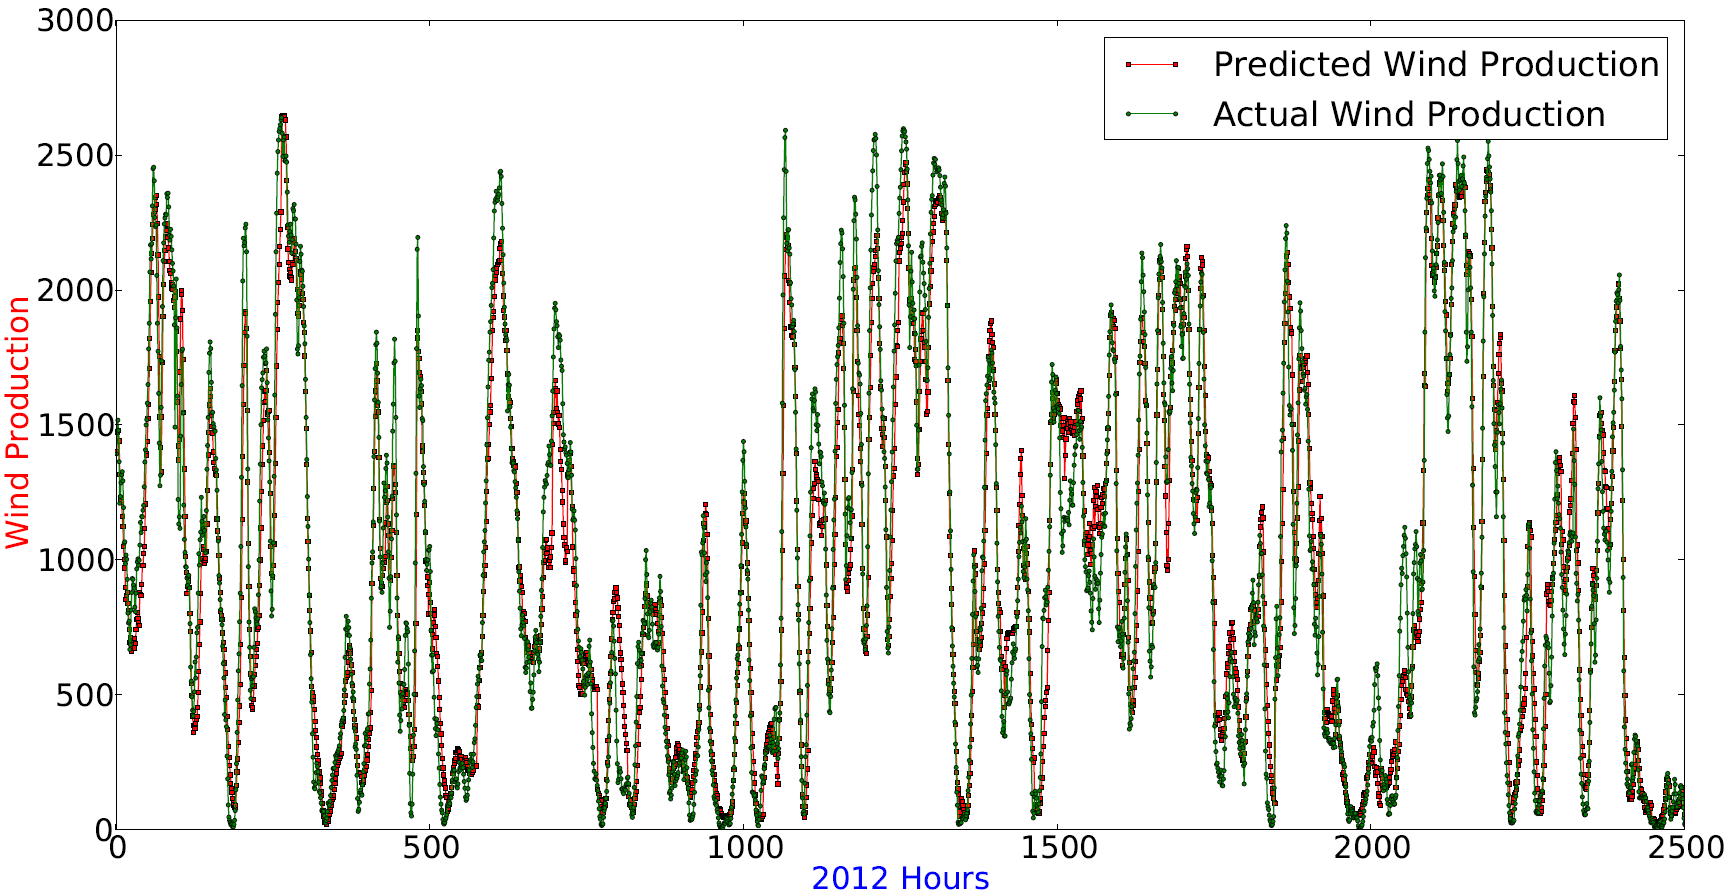
\includegraphics[width=0.99\linewidth]{billeder/bestInputCombi0-2500.png}
\caption{Wind Power prediction for 0-2500 hours in 2012 with the best combination}
\label{fig:bestInputCombi0-2500}
\end{sidewaysfigure} 

\begin{sidewaysfigure}[h!]
\centering
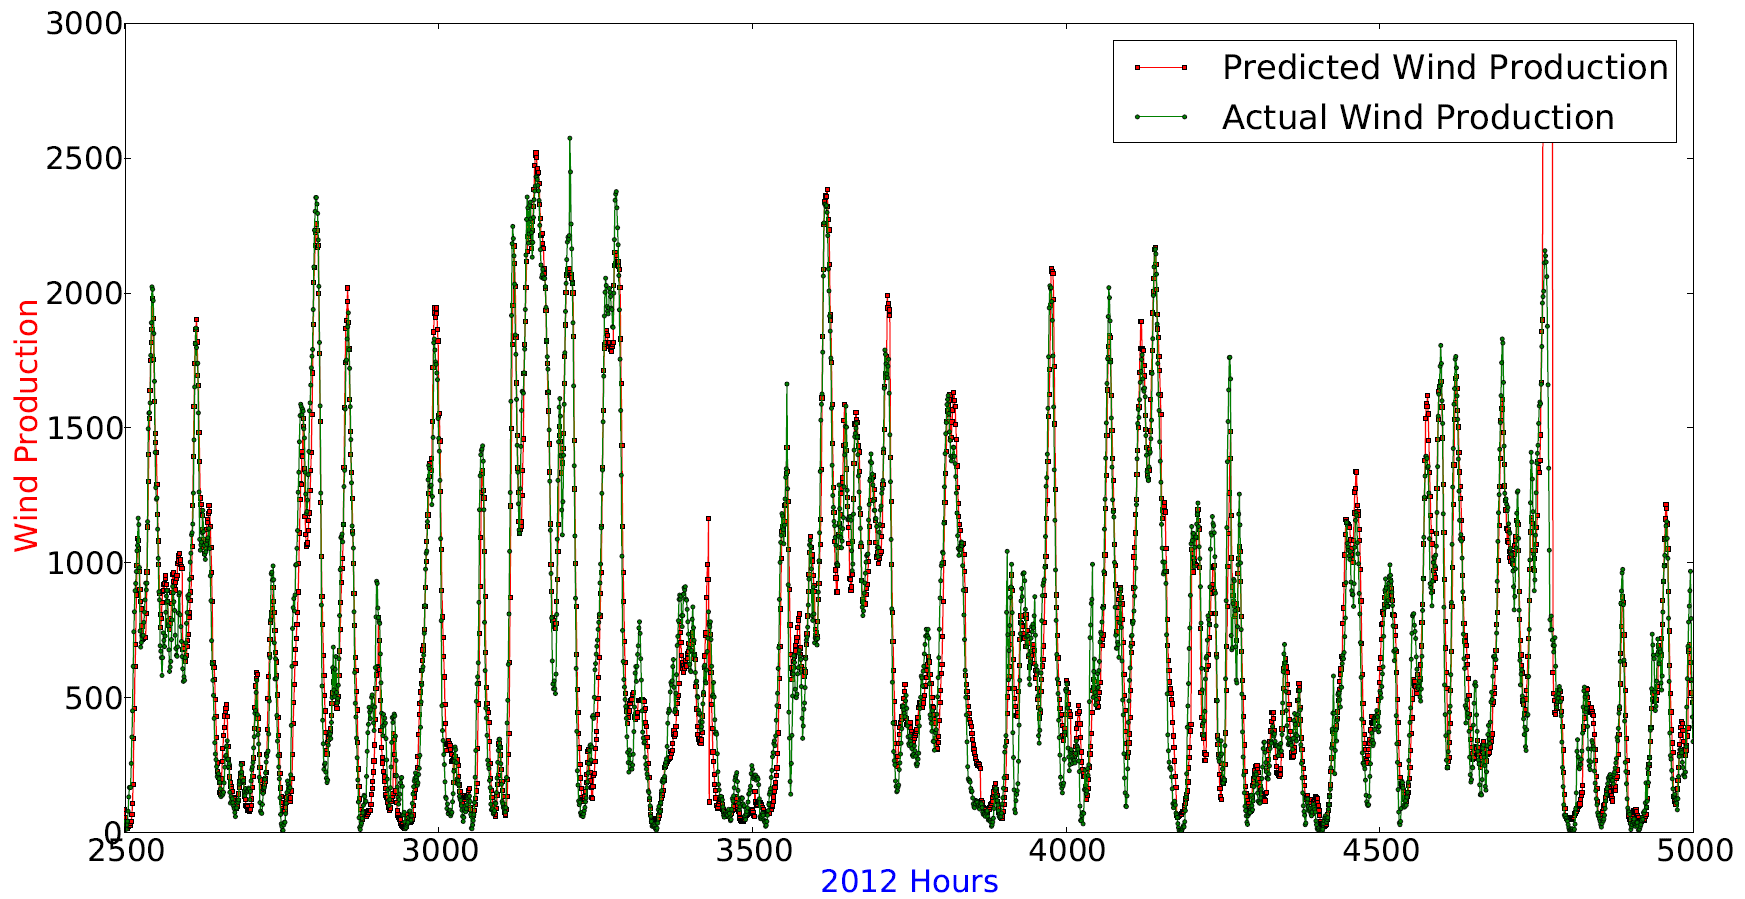
\includegraphics[width=0.99\linewidth]{billeder/bestInputCombi2500-5000.png}
\caption{Wind Power prediction for 2500-5000 hours in 2012 with the best combination}
\label{fig:bestInputCombi2500-5000}
\end{sidewaysfigure} 

\subsubsection{Simple input test with seasonality}
\label{sec:simpleInputTestSeason}
The simple input test based on 3 months before the prediction day and the same month in the previous year. All with 200 epochs.

WS = Wind Speed
AD = Air Density
C = Consumption
T = Temperature
WD = Wind Direction
L-P = Last Known Production
D = Date
ToD = Time of Day
M = Time of Day as matrix
CD = Correct direction in \%

\footnotesize
\begin{center}
\begin{longtable}{|c|c|c|c|c|c|c|c|c|c|c|c|c|}
\caption{Wind Production Input Parameter Test}\\
\hline
\textbf{WS} & \textbf{AD} & \textbf{C} & \textbf{T} & \textbf{WD} & \textbf{L-P} & \textbf{D}& \textbf{ToD} & \textbf{MAE} & \textbf{\% from \#1} & \textbf{H1} & \textbf{H2} & \textbf{H2} \\
\hline
\endfirsthead
\multicolumn{13}{c}%
{\tablename\ \thetable\ -- \textit{Continued from previous page}} \\
\hline
\textbf{WS} & \textbf{AD} & \textbf{C} & \textbf{T} & \textbf{WD} & \textbf{L-P} & \textbf{D}& \textbf{ToD} & \textbf{MAE} & \textbf{\% from \#1} & \textbf{H1} & \textbf{H2} & \textbf{CD} \\
\hline
\endhead
\hline \multicolumn{13}{r}{\textit{Continued on next page}} \\
\endfoot
\hline
\endlastfoot
\arrayrulecolor{light-gray}
 \x &  \x &  \x &  &  \x &  \x &  &  \x & 142,88 & 0,0\% & 7 & 17 & 73\% \\ \hline
 \x &  &  &  \x &  \x &  \x &  &  \x & 142,89 & 0,01\% & 14 & 11 & 73\% \\ \hline
 \x &  \x &  &  &  \x &  \x &  &  \x & 143,37 & 0,34\% & 3 & 21 & 73\% \\ \hline
 \x &  \x &  \x &  \x &  \x &  \x &  &  \x & 143,97 & 0,76\% & 4 & 25 & 72\% \\ \hline
 \x &  &  &  &  &  \x &  &  \x & 143,98 & 0,77\% & 2 & 21 & 72\% \\ \hline
 \x &  \x &  \x &  \x &  &  \x &  \x &  \x & 144,11 & 0,86\% & 1 & 17 & 73\% \\ \hline
 \x &  \x &  &  &  &  \x &  &  \x & 144,12 & 0,87\% & 7 & 12 & 73\% \\ \hline
 \x &  &  &  &  &  &  &  \x & 144,28 & 0,98\% & 12 & 17 & 41\% \\ \hline
 \x &  &  \x &  &  \x &  \x &  &  \x & 144,42 & 1,08\% & 11 & 10 & 72\% \\ \hline
 \x &  \x &  &  \x &  \x &  \x &  &  \x & 144,48 & 1,12\% & 1 & 17 & 73\% \\ \hline
 \x &  &  \x &  \x &  &  \x &  &  \x & 144,7 & 1,27\% & 21 & 6 & 72\% \\ \hline
 \x &  \x &  \x &  \x &  &  \x &  &  \x & 144,79 & 1,34\% & 18 & 13 & 72\% \\ \hline
 \x &  &  &  &  &  \x &  &  \x & 144,93 & 1,43\% & 18 & 1 & 73\% \\ \hline
 \x &  &  \x &  \x &  \x &  \x &  \x &  \x & 144,98 & 1,47\% & 14 & 9 & 73\% \\ \hline
 \x &  &  \x &  \x &  &  \x &  \x &  \x & 145,02 & 1,5\% & 18 & 11 & 73\% \\ \hline
 \x &  \x &  \x &  \x &  &  \x &  \x &  \x & 145,19 & 1,62\% & 2 & 15 & 73\% \\ \hline
 \x &  &  &  \x &  &  \x &  \x &  \x & 145,29 & 1,69\% & 13 & 6 & 73\% \\ \hline
 \x &  \x &  &  &  &  &  &  \x & 145,51 & 1,84\% & 1 & 22 & 54\% \\ \hline
 \x &  &  \x &  &  \x &  \x &  &  \x & 145,76 & 2,02\% & 13 & 17 & 73\% \\ \hline
 \x &  \x &  \x &  &  \x &  &  &  \x & 145,79 & 2,04\% & 18 & 9 & 62\% \\ \hline
 \x &  \x &  \x &  &  \x &  \x &  \x &  \x & 145,98 & 2,17\% & 1 & 9 & 73\% \\ \hline
 \x &  &  \x &  &  &  &  &  \x & 145,99 & 2,18\% & 16 & 13 & 64\% \\ \hline
 \x &  &  &  &  \x &  &  &  \x & 146,24 & 2,35\% & 24 & 9 & 61\% \\ \hline
 \x &  \x &  \x &  &  \x &  \x &  &  \x & 146,49 & 2,53\% & 2 & 13 & 72\% \\ \hline
 \x &  &  \x &  &  &  \x &  &  \x & 146,53 & 2,55\% & 1 & 18 & 73\% \\ \hline
 \x &  \x &  \x &  &  &  &  &  \x & 146,57 & 2,58\% & 24 & 11 & 64\% \\ \hline
 \x &  \x &  \x &  &  \x &  \x &  \x &  \x & 146,61 & 2,61\% & 5 & 15 & 72\% \\ \hline
 \x &  \x &  &  \x &  \x &  \x &  \x &  \x & 146,64 & 2,63\% & 1 & 13 & 73\% \\ \hline
 \x &  \x &  \x &  \x &  \x &  \x &  \x &  \x & 146,78 & 2,73\% & 2 & 16 & 73\% \\ \hline
 \x &  \x &  \x &  \x &  \x &  \x &  \x &  \x & 146,89 & 2,81\% & 4 & 16 & 72\% \\ \hline
 \x &  \x &  &  &  &  &  &  \x & 146,96 & 2,86\% & 25 & 5 & 54\% \\ \hline
 \x &  \x &  \x &  &  &  \x &  &  \x & 147,18 & 3,01\% & 14 & 15 & 72\% \\ \hline
 \x &  &  \x &  \x &  &  \x &  &  \x & 147,3 & 3,09\% & 17 & 7 & 72\% \\ \hline
 \x &  &  &  &  &  \x &  \x &  \x & 147,64 & 3,33\% & 11 & 11 & 73\% \\ \hline
 \x &  &  \x &  &  &  &  &  \x & 147,7 & 3,37\% & 11 & 22 & 63\% \\ \hline
 \x &  \x &  \x &  &  &  &  &  \x & 147,86 & 3,49\% & 10 & 25 & 63\% \\ \hline
 \x &  &  &  &  \x &  \x &  \x &  \x & 147,95 & 3,55\% & 4 & 17 & 73\% \\ \hline
 \x &  &  \x &  &  &  \x &  &  \x & 147,98 & 3,57\% & 14 & 17 & 72\% \\ \hline
 \x &  &  &  &  \x &  \x &  \x &  \x & 148,23 & 3,74\% & 1 & 23 & 73\% \\ \hline
 \x &  \x &  &  \x &  &  \x &  \x &  \x & 148,28 & 3,78\% & 5 & 13 & 73\% \\ \hline
 \x &  &  &  \x &  \x &  \x &  \x &  \x & 148,4 & 3,86\% & 13 & 13 & 73\% \\ \hline
 \x &  \x &  &  \x &  &  \x &  &  \x & 148,57 & 3,98\% & 21 & 14 & 72\% \\ \hline
 \x &  \x &  \x &  \x &  &  &  &  \x & 148,66 & 4,05\% & 14 & 20 & 63\% \\ \hline
 \x &  \x &  \x &  \x &  &  &  &  \x & 149,0 & 4,28\% & 7 & 25 & 63\% \\ \hline
 \x &  \x &  &  &  \x &  &  &  \x & 149,04 & 4,31\% & 16 & 12 & 61\% \\ \hline
 \x &  &  &  \x &  &  \x &  &  \x & 149,08 & 4,34\% & 19 & 15 & 72\% \\ \hline
 \x &  &  \x &  &  &  \x &  \x &  \x & 149,13 & 4,37\% & 3 & 16 & 73\% \\ \hline
 \x &  \x &  \x &  &  &  \x &  \x &  \x & 149,28 & 4,48\% & 2 & 16 & 73\% \\ \hline
 \x &  \x &  &  \x &  \x &  \x &  &  \x & 149,31 & 4,5\% & 1 & 17 & 72\% \\ \hline
 \x &  &  \x &  &  \x &  &  &  \x & 149,4 & 4,56\% & 14 & 18 & 63\% \\ \hline
 \x &  \x &  \x &  &  &  \x &  &  \x & 149,95 & 4,95\% & 1 & 16 & 73\% \\ \hline
 \x &  &  \x &  &  \x &  \x &  \x &  \x & 150,28 & 5,18\% & 1 & 22 & 72\% \\ \hline
 \x &  \x &  \x &  \x &  &  \x &  &  \x & 150,33 & 5,21\% & 9 & 19 & 72\% \\ \hline
 \x &  \x &  &  &  &  \x &  \x &  \x & 150,36 & 5,24\% & 4 & 15 & 73\% \\ \hline
 \x &  \x &  &  &  &  \x &  &  \x & 150,98 & 5,67\% & 21 & 1 & 72\% \\ \hline
 \x &  &  &  &  \x &  &  &  \x & 151,09 & 5,75\% & 11 & 21 & 61\% \\ \hline
 \x &  &  \x &  \x &  &  &  &  \x & 151,13 & 5,77\% & 20 & 10 & 63\% \\ \hline
 \x &  &  &  \x &  &  &  &  \x & 151,3 & 5,89\% & 20 & 15 & 50\% \\ \hline
 \x &  \x &  &  \x &  &  \x &  &  \x & 151,45 & 6,0\% & 7 & 20 & 72\% \\ \hline
 \x &  \x &  \x &  \x &  \x &  \x &  &  \x & 151,46 & 6,01\% & 10 & 24 & 72\% \\ \hline
 \x &  \x &  &  &  \x &  \x &  \x &  \x & 151,48 & 6,02\% & 2 & 16 & 73\% \\ \hline
 \x &  \x &  &  \x &  \x &  \x &  \x &  \x & 151,67 & 6,15\% & 4 & 17 & 72\% \\ \hline
 \x &  &  \x &  \x &  &  &  &  \x & 151,7 & 6,17\% & 17 & 13 & 63\% \\ \hline
 \x &  &  \x &  \x &  \x &  \x &  \x &  \x & 151,76 & 6,22\% & 2 & 16 & 72\% \\ \hline
 \x &  &  \x &  \x &  \x &  \x &  &  \x & 151,91 & 6,32\% & 1 & 9 & 71\% \\ \hline
 \x &  &  \x &  \x &  &  \x &  \x &  \x & 152,06 & 6,42\% & 7 & 22 & 72\% \\ \hline
 \x &  \x &  &  &  \x &  &  &  \x & 152,25 & 6,56\% & 19 & 12 & 61\% \\ \hline
 \x &  &  &  &  \x &  \x &  &  \x & 152,28 & 6,58\% & 19 & 14 & 72\% \\ \hline
 \x &  \x &  &  \x &  &  &  &  \x & 152,35 & 6,63\% & 23 & 12 & 54\% \\ \hline
 \x &  \x &  &  &  &  \x &  \x &  \x & 152,36 & 6,63\% & 10 & 22 & 73\% \\ \hline
 \x &  \x &  \x &  \x &  \x &  &  \x &  \x & 152,39 & 6,66\% & 18 & 9 & 63\% \\ \hline
 \x &  &  &  \x &  \x &  \x &  &  \x & 152,43 & 6,68\% & 6 & 23 & 72\% \\ \hline
 \x &  \x &  &  &  \x &  \x &  &  \x & 153,17 & 7,2\% & 2 & 10 & 72\% \\ \hline
 \x &  \x &  \x &  &  &  &  \x &  \x & 153,2 & 7,22\% & 7 & 13 & 63\% \\ \hline
 \x &  &  \x &  \x &  \x &  &  \x &  \x & 153,3 & 7,29\% & 13 & 20 & 63\% \\ \hline
 \x &  &  \x &  \x &  &  &  \x &  \x & 153,52 & 7,45\% & 16 & 15 & 63\% \\ \hline
 \x &  &  &  \x &  &  &  &  \x & 153,6 & 7,5\% & 22 & 14 & 51\% \\ \hline
 \x &  \x &  \x &  &  &  \x &  \x &  \x & 153,82 & 7,66\% & 8 & 14 & 73\% \\ \hline
 \x &  &  \x &  \x &  \x &  &  &  \x & 153,84 & 7,67\% & 9 & 20 & 62\% \\ \hline
 \x &  &  &  &  \x &  \x &  &  \x & 153,95 & 7,75\% & 15 & 12 & 73\% \\ \hline
 \x &  &  \x &  &  \x &  &  &  \x & 154,16 & 7,89\% & 14 & 13 & 61\% \\ \hline
 \x &  \x &  &  \x &  &  &  &  \x & 154,18 & 7,91\% & 12 & 24 & 54\% \\ \hline
 \x &  \x &  \x &  \x &  &  &  \x &  \x & 154,84 & 8,37\% & 13 & 18 & 63\% \\ \hline
 \x &  &  &  \x &  \x &  \x &  \x &  \x & 154,94 & 8,44\% & 1 & 18 & 72\% \\ \hline
 \x &  \x &  \x &  \x &  &  &  \x &  \x & 154,95 & 8,45\% & 2 & 21 & 62\% \\ \hline
 \x &  \x &  &  \x &  &  &  \x &  \x & 155,0 & 8,48\% & 18 & 12 & 54\% \\ \hline
 \x &  &  &  &  &  &  &  \x & 155,07 & 8,53\% & 7 & 21 & 41\% \\ \hline
 \x &  \x &  \x &  &  \x &  &  \x &  \x & 155,46 & 8,8\% & 16 & 15 & 63\% \\ \hline
 \x &  &  \x &  \x &  \x &  &  \x &  \x & 155,7 & 8,97\% & 16 & 18 & 62\% \\ \hline
 \x &  \x &  \x &  \x &  \x &  &  &  \x & 155,79 & 9,04\% & 19 & 11 & 62\% \\ \hline
 \x &  \x &  \x &  &  &  &  \x &  \x & 155,82 & 9,06\% & 7 & 22 & 62\% \\ \hline
 \x &  &  \x &  \x &  &  &  \x &  \x & 155,89 & 9,11\% & 13 & 22 & 63\% \\ \hline
 \x &  \x &  &  &  &  &  \x &  \x & 156,04 & 9,21\% & 22 & 8 & 54\% \\ \hline
 \x &  &  &  \x &  &  \x &  &  \x & 156,14 & 9,28\% & 1 & 21 & 72\% \\ \hline
 \x &  \x &  &  &  \x &  &  \x &  \x & 156,34 & 9,42\% & 14 & 16 & 61\% \\ \hline
 \x &  &  &  \x &  \x &  &  \x &  \x & 156,59 & 9,6\% & 12 & 22 & 61\% \\ \hline
 \x &  &  &  &  &  \x &  \x &  \x & 156,6 & 9,6\% & 22 & 1 & 72\% \\ \hline
 \x &  &  \x &  &  \x &  \x &  \x &  \x & 156,84 & 9,77\% & 1 & 10 & 71\% \\ \hline
 \x &  &  \x &  &  &  &  \x &  \x & 156,89 & 9,81\% & 14 & 19 & 62\% \\ \hline
 \x &  \x &  &  \x &  \x &  &  \x &  \x & 157,48 & 10,22\% & 12 & 17 & 61\% \\ \hline
 \x &  &  &  \x &  &  &  \x &  \x & 157,61 & 10,31\% & 15 & 14 & 50\% \\ \hline
 \x &  &  &  \x &  \x &  &  &  \x & 158,37 & 10,84\% & 25 & 9 & 60\% \\ \hline
 \x &  \x &  &  &  \x &  &  \x &  \x & 158,46 & 10,9\% & 5 & 23 & 61\% \\ \hline
 \x &  \x &  &  \x &  \x &  &  &  \x & 158,64 & 11,03\% & 22 & 9 & 61\% \\ \hline
 \x &  \x &  &  &  &  &  \x &  \x & 158,74 & 11,1\% & 24 & 1 & 54\% \\ \hline
 \x &  \x &  &  &  \x &  \x &  \x &  \x & 159,01 & 11,29\% & 2 & 23 & 72\% \\ \hline
 \x &  &  \x &  &  \x &  &  \x &  \x & 159,25 & 11,46\% & 12 & 23 & 62\% \\ \hline
 \x &  \x &  \x &  \x &  \x &  &  \x &  \x & 159,32 & 11,51\% & 14 & 24 & 62\% \\ \hline
 \x &  \x &  \x &  &  \x &  &  \x &  \x & 159,44 & 11,59\% & 14 & 12 & 63\% \\ \hline
 \x &  &  \x &  &  &  \x &  \x &  \x & 159,6 & 11,7\% & 2 & 13 & 71\% \\ \hline
 \x &  \x &  \x &  &  \x &  &  &  \x & 159,74 & 11,8\% & 12 & 14 & 61\% \\ \hline
 \x &  &  &  \x &  &  &  \x &  \x & 159,94 & 11,94\% & 11 & 15 & 51\% \\ \hline
 \x &  \x &  &  \x &  &  \x &  \x &  \x & 160,11 & 12,06\% & 10 & 14 & 71\% \\ \hline
 \x &  \x &  \x &  \x &  \x &  &  &  \x & 160,55 & 12,37\% & 15 & 19 & 62\% \\ \hline
 \x &  &  &  &  \x &  &  \x &  \x & 160,79 & 12,53\% & 17 & 13 & 61\% \\ \hline
 \x &  &  &  &  &  &  \x &  \x & 160,98 & 12,67\% & 10 & 21 & 41\% \\ \hline
 \x &  \x &  &  \x &  \x &  &  \x &  \x & 161,12 & 12,77\% & 13 & 13 & 61\% \\ \hline
 \x &  &  &  &  &  &  \x &  \x & 161,18 & 12,81\% & 18 & 12 & 41\% \\ \hline
 \x &  &  \x &  &  &  &  \x &  \x & 161,25 & 12,86\% & 3 & 25 & 62\% \\ \hline
 \x &  &  \x &  \x &  \x &  &  &  \x & 161,5 & 13,03\% & 18 & 17 & 62\% \\ \hline
 \x &  &  &  &  \x &  &  \x &  \x & 161,59 & 13,09\% & 16 & 20 & 60\% \\ \hline
 \x &  \x &  &  \x &  &  &  \x &  \x & 162,1 & 13,45\% & 6 & 22 & 54\% \\ \hline
 \x &  &  \x &  &  \x &  &  \x &  \x & 162,54 & 13,76\% & 12 & 13 & 62\% \\ \hline
 \x &  \x &  &  \x &  \x &  &  &  \x & 162,55 & 13,77\% & 19 & 15 & 60\% \\ \hline
 \x &  &  &  \x &  &  \x &  \x &  \x & 162,57 & 13,78\% & 4 & 23 & 71\% \\ \hline
 \x &  &  &  \x &  \x &  &  &  \x & 162,87 & 13,99\% & 15 & 19 & 60\% \\ \hline
 \x &  &  &  \x &  \x &  &  \x &  \x & 163,34 & 14,32\% & 15 & 19 & 61\% \\ \hline
 \x &  &  \x &  \x &  \x &  \x &  &  \x & 165,37 & 15,74\% & 13 & 18 & 71\% \\ \hline
\end{longtable}
\label{table:windProdInputParamsSeasonal}
\end{center}
\normalsize

\footnotesize
\begin{center}
\begin{longtable}{|c|c|c|c|}
\hline
\textbf{MAPE (unseen data)} \textbf{MAE (unseen data)} & \textbf{MAE (training set)} & \textbf{MAPE (training set)}  \\
\hline
\endfirsthead
\multicolumn{4}{c}%
{\tablename\ \thetable\ -- \textit{Continued from previous page}} \\
\hline
\textbf{MAPE (unseen data)} \textbf{MAE (unseen data)} & \textbf{MAE (training set)} & \textbf{MAPE (training set)}  \\
\hline
\endhead
\hline \multicolumn{4}{r}{\textit{Continued on next page}} \\
\endfoot
\hline
\endlastfoot
\arrayrulecolor{light-gray}
21.44\% 142,88 & 51.17 & 7.68\%  \\ \hline
21.44\% 142,89 & 50.08 & 7.51\%  \\ \hline
21.51\% 143,37 & 52.01 & 7.8\%  \\ \hline
21.6\% 143,97 & 48.2 & 7.23\%  \\ \hline
21.6\% 143,98 & 49.51 & 7.43\%  \\ \hline
21.62\% 144,11 & 49.31 & 7.4\%  \\ \hline
21.62\% 144,12 & 49.29 & 7.4\%  \\ \hline
21.65\% 144,28 & 121.29 & 18.2\%  \\ \hline
21.67\% 144,42 & 50.5 & 7.58\%  \\ \hline
21.68\% 144,48 & 47.67 & 7.15\%  \\ \hline
21.71\% 144,7 & 47.6 & 7.14\%  \\ \hline
21.72\% 144,79 & 47.25 & 7.09\%  \\ \hline
21.74\% 144,93 & 51.33 & 7.7\%  \\ \hline
21.75\% 144,98 & 47.8 & 7.17\%  \\ \hline
21.76\% 145,02 & 47.83 & 7.18\%  \\ \hline
21.78\% 145,19 & 49.59 & 7.44\%  \\ \hline
21.8\% 145,29 & 52.35 & 7.85\%  \\ \hline
21.83\% 145,51 & 119.38 & 17.91\%  \\ \hline
21.87\% 145,76 & 51.67 & 7.75\%  \\ \hline
21.87\% 145,79 & 107.59 & 16.14\%  \\ \hline
21.9\% 145,98 & 51.89 & 7.79\%  \\ \hline
21.9\% 145,99 & 119.02 & 17.86\%  \\ \hline
21.94\% 146,24 & 106.17 & 15.93\%  \\ \hline
21.98\% 146,49 & 51.22 & 7.68\%  \\ \hline
21.98\% 146,53 & 49.0 & 7.35\%  \\ \hline
21.99\% 146,57 & 116.61 & 17.5\%  \\ \hline
22.0\% 146,61 & 49.56 & 7.44\%  \\ \hline
22.0\% 146,64 & 53.11 & 7.97\%  \\ \hline
22.02\% 146,78 & 48.35 & 7.25\%  \\ \hline
22.04\% 146,89 & 46.8 & 7.02\%  \\ \hline
22.05\% 146,96 & 116.64 & 17.5\%  \\ \hline
22.08\% 147,18 & 49.79 & 7.47\%  \\ \hline
22.1\% 147,3 & 49.44 & 7.42\%  \\ \hline
22.15\% 147,64 & 53.91 & 8.09\%  \\ \hline
22.16\% 147,7 & 117.07 & 17.56\%  \\ \hline
22.18\% 147,86 & 114.41 & 17.17\%  \\ \hline
22.2\% 147,95 & 49.69 & 7.46\%  \\ \hline
22.2\% 147,98 & 50.62 & 7.59\%  \\ \hline
22.24\% 148,23 & 54.92 & 8.24\%  \\ \hline
22.25\% 148,28 & 47.43 & 7.12\%  \\ \hline
22.27\% 148,4 & 50.55 & 7.58\%  \\ \hline
22.29\% 148,57 & 47.97 & 7.2\%  \\ \hline
22.3\% 148,66 & 103.73 & 15.56\%  \\ \hline
22.36\% 149,0 & 102.43 & 15.37\%  \\ \hline
22.36\% 149,04 & 111.43 & 16.72\%  \\ \hline
22.37\% 149,08 & 50.89 & 7.64\%  \\ \hline
22.38\% 149,13 & 52.85 & 7.93\%  \\ \hline
22.4\% 149,28 & 48.54 & 7.28\%  \\ \hline
22.4\% 149,31 & 47.08 & 7.06\%  \\ \hline
22.42\% 149,4 & 110.64 & 16.6\%  \\ \hline
22.5\% 149,95 & 51.21 & 7.68\%  \\ \hline
22.55\% 150,28 & 50.56 & 7.59\%  \\ \hline
22.56\% 150,33 & 49.2 & 7.38\%  \\ \hline
22.56\% 150,36 & 55.02 & 8.26\%  \\ \hline
22.65\% 150,98 & 50.5 & 7.58\%  \\ \hline
22.67\% 151,09 & 108.91 & 16.34\%  \\ \hline
22.68\% 151,13 & 103.18 & 15.48\%  \\ \hline
22.7\% 151,3 & 106.54 & 15.98\%  \\ \hline
22.72\% 151,45 & 49.75 & 7.46\%  \\ \hline
22.72\% 151,46 & 49.75 & 7.46\%  \\ \hline
22.73\% 151,48 & 49.15 & 7.37\%  \\ \hline
22.76\% 151,67 & 48.98 & 7.35\%  \\ \hline
22.76\% 151,7 & 102.61 & 15.4\%  \\ \hline
22.77\% 151,76 & 52.56 & 7.89\%  \\ \hline
22.79\% 151,91 & 47.06 & 7.06\%  \\ \hline
22.81\% 152,06 & 54.21 & 8.13\%  \\ \hline
22.84\% 152,25 & 104.83 & 15.73\%  \\ \hline
22.85\% 152,28 & 49.39 & 7.41\%  \\ \hline
22.86\% 152,35 & 106.83 & 16.03\%  \\ \hline
22.86\% 152,36 & 56.15 & 8.42\%  \\ \hline
22.86\% 152,39 & 98.23 & 14.74\%  \\ \hline
22.87\% 152,43 & 48.38 & 7.26\%  \\ \hline
22.98\% 153,17 & 49.06 & 7.36\%  \\ \hline
22.99\% 153,2 & 108.27 & 16.24\%  \\ \hline
23.0\% 153,3 & 95.73 & 14.36\%  \\ \hline
23.03\% 153,52 & 100.28 & 15.05\%  \\ \hline
23.05\% 153,6 & 106.84 & 16.03\%  \\ \hline
23.08\% 153,82 & 50.63 & 7.6\%  \\ \hline
23.08\% 153,84 & 99.64 & 14.95\%  \\ \hline
23.1\% 153,95 & 48.48 & 7.27\%  \\ \hline
23.13\% 154,16 & 104.68 & 15.71\%  \\ \hline
23.13\% 154,18 & 107.35 & 16.11\%  \\ \hline
23.23\% 154,84 & 98.24 & 14.74\%  \\ \hline
23.25\% 154,94 & 51.48 & 7.72\%  \\ \hline
23.25\% 154,95 & 104.48 & 15.68\%  \\ \hline
23.26\% 155,0 & 116.53 & 17.48\%  \\ \hline
23.27\% 155,07 & 120.01 & 18.01\%  \\ \hline
23.32\% 155,46 & 97.84 & 14.68\%  \\ \hline
23.36\% 155,7 & 101.32 & 15.2\%  \\ \hline
23.37\% 155,79 & 99.4 & 14.91\%  \\ \hline
23.38\% 155,82 & 117.43 & 17.62\%  \\ \hline
23.39\% 155,89 & 102.64 & 15.4\%  \\ \hline
23.41\% 156,04 & 114.04 & 17.11\%  \\ \hline
23.43\% 156,14 & 47.18 & 7.08\%  \\ \hline
23.46\% 156,34 & 114.25 & 17.14\%  \\ \hline
23.49\% 156,59 & 100.22 & 15.04\%  \\ \hline
23.5\% 156,6 & 51.23 & 7.69\%  \\ \hline
23.53\% 156,84 & 50.49 & 7.58\%  \\ \hline
23.54\% 156,89 & 111.68 & 16.76\%  \\ \hline
23.63\% 157,48 & 109.58 & 16.44\%  \\ \hline
23.65\% 157,61 & 97.65 & 14.65\%  \\ \hline
23.76\% 158,37 & 98.79 & 14.82\%  \\ \hline
23.77\% 158,46 & 100.89 & 15.14\%  \\ \hline
23.8\% 158,64 & 100.0 & 15.0\%  \\ \hline
23.82\% 158,74 & 113.42 & 17.02\%  \\ \hline
23.86\% 159,01 & 54.71 & 8.21\%  \\ \hline
23.89\% 159,25 & 102.77 & 15.42\%  \\ \hline
23.9\% 159,32 & 97.86 & 14.68\%  \\ \hline
23.92\% 159,44 & 102.8 & 15.42\%  \\ \hline
23.95\% 159,6 & 51.08 & 7.66\%  \\ \hline
23.97\% 159,74 & 102.87 & 15.43\%  \\ \hline
24.0\% 159,94 & 104.03 & 15.61\%  \\ \hline
24.02\% 160,11 & 48.17 & 7.23\%  \\ \hline
24.09\% 160,55 & 102.1 & 15.32\%  \\ \hline
24.12\% 160,79 & 107.84 & 16.18\%  \\ \hline
24.15\% 160,98 & 112.07 & 16.81\%  \\ \hline
24.17\% 161,12 & 106.74 & 16.02\%  \\ \hline
24.18\% 161,18 & 114.86 & 17.23\%  \\ \hline
24.19\% 161,25 & 115.31 & 17.3\%  \\ \hline
24.23\% 161,5 & 95.21 & 14.29\%  \\ \hline
24.24\% 161,59 & 107.01 & 16.06\%  \\ \hline
24.32\% 162,1 & 107.47 & 16.12\%  \\ \hline
24.39\% 162,54 & 104.96 & 15.75\%  \\ \hline
24.39\% 162,55 & 105.16 & 15.78\%  \\ \hline
24.39\% 162,57 & 49.9 & 7.49\%  \\ \hline
24.44\% 162,87 & 99.29 & 14.9\%  \\ \hline
24.51\% 163,34 & 97.13 & 14.57\%  \\ \hline
24.81\% 165,37 & 50.1 & 7.52\%  \\ \hline
\caption{Average prediction MAE/MAPE on unseen data vs. prediction MAE/MAPE on training set for season}
\label{table:predictionMAEUnseenVsTrainingSetSeasonAppendix}
\end{longtable}
\end{center}
\normalsize
\subsection{Experiment two}

\subsubsection{Historical volatility results}
\label{sec:historicalVolatiltiyResultsAppendix}
Historical volatility results with all combinations of previous hours between 4-24 and different smoothing factors.

\footnotesize
\begin{center}
\begin{longtable}{|c|c|c|c|}
\caption{Wind Production Input Parameter Test}\\
\hline
\textbf{Previous Hours} & \textbf{Smoothing factor} & \textbf{MAE} & \textbf{\% Deviation} \\
\hline
\endfirsthead
\multicolumn{4}{c}%
{\tablename\ \thetable\ -- \textit{Continued from previous page}} \\
\hline
\textbf{Previous Hours} & \textbf{Smoothing factor} & \textbf{MAE} & \textbf{\% Deviation} \\
\hline
\endhead
\hline \multicolumn{4}{r}{\textit{Continued on next page}} \\
\endfoot
\hline
\endlastfoot
\arrayrulecolor{light-gray}
6 & 0,70 & 121,81 & 0,0\% \\ \hline
20 & 0,80 & 122,9 & 0,89\% \\ \hline
24 & 0,60 & 123,13 & 1,08\% \\ \hline
24 & 0,80 & 124,02 & 1,81\% \\ \hline
16 & 0,20 & 125,65 & 3,15\% \\ \hline
12 & 0,30 & 127,0 & 4,26\% \\ \hline
24 & 0,70 & 127,06 & 4,31\% \\ \hline
16 & 0, 60 & 127,38 & 4,57\% \\ \hline
24 & 0,40 & 127,51 & 4,68\% \\ \hline
16 & 0,90 & 127,77 & 4,89\% \\ \hline
16 & 0,30 & 127,86 & 4,97\% \\ \hline
4 & 0,60 & 128,49 & 5,48\% \\ \hline
4 & 0,10 & 128,51 & 5,5\% \\ \hline
20 & 0,50 & 129,36 & 6,2\% \\ \hline
8 & 0,10 & 130,06 & 6,77\% \\ \hline
24 & 0,20 & 131,05 & 7,59\% \\ \hline
12 & 0,90 & 131,87 & 8,26\% \\ \hline
20 & 0,10 & 132,63 & 8,88\% \\ \hline
20 & 0,30 & 133,32 & 9,45\% \\ \hline
6 & 0,20 & 133,67 & 9,74\% \\ \hline
4 & 0,30 & 133,84 & 9,88\% \\ \hline
12 & 0,60 & 134,02 & 10,02\% \\ \hline
4 & 0,20 & 134,18 & 10,16\% \\ \hline
16 & 0,40 & 134,28 & 10,24\% \\ \hline
4 & 0,40 & 134,71 & 10,59\% \\ \hline
12 & 0,40 & 135,05 & 10,87\% \\ \hline
16 & 0,80 & 135,14 & 10,94\% \\ \hline
20 & 0,20 & 135,3 & 11,07\% \\ \hline
12 & 0,50 & 135,42 & 11,17\% \\ \hline
24 & 0,90 & 135,71 & 11,41\% \\ \hline
16 & 0,50 & 136,44 & 12,01\% \\ \hline
4 & 0,50 & 136,58 & 12,13\% \\ \hline
6 & 0,30 & 136,6 & 12,14\% \\ \hline
20 & 0,70 & 136,63 & 12,17\% \\ \hline
20 & 0,60 & 136,86 & 12,36\% \\ \hline
12 & 0,20 & 136,98 & 12,45\% \\ \hline
6 & 0,10 & 137,16 & 12,6\% \\ \hline
24 & 0,10 & 137,34 & 12,75\% \\ \hline
6 & 0,50 & 137,45 & 12,84\% \\ \hline
24 & 0,50 & 137,91 & 13,22\% \\ \hline
20 & 0,90 & 137,92 & 13,23\% \\ \hline
8 & 0,20 & 138,26 & 13,5\% \\ \hline
8 & 0,40 & 138,69 & 13,86\% \\ \hline
6 & 0,60 & 138,87 & 14,01\% \\ \hline
8 & 0,50 & 138,93 & 14,05\% \\ \hline
8 & 0,60 & 139,2 & 14,28\% \\ \hline
8 & 0,90 & 139,84 & 14,8\% \\ \hline
8 & 0,70 & 140,01 & 14,94\% \\ \hline
24 & 0,30 & 140,45 & 15,3\% \\ \hline
6 & 0,70 & 141,3 & 16,0\% \\ \hline
8 & 0,30 & 141,6 & 16,25\% \\ \hline
4 & 0,70 & 142,19 & 16,73\% \\ \hline
12 & 0,80 & 142,2 & 16,74\% \\ \hline
6 & 0,40 & 142,98 & 17,38\% \\ \hline
6 & 0,80 & 143,21 & 17,57\% \\ \hline
20 & 0,40 & 143,59 & 17,88\% \\ \hline
8 & 0,80 & 143,62 & 17,9\% \\ \hline
12 & 0,10 & 144,37 & 18,52\% \\ \hline
16 & 0,70 & 144,43 & 18,57\% \\ \hline
16 & 0,10 & 146,77 & 20,49\% \\ \hline
4 & 0,80 & 146,9 & 20,6\% \\ \hline
6 & 0,90 & 147,48 & 21,07\% \\ \hline
4 & 0,90 & 151,15 & 24,09\% \\ \hline
\end{longtable}
\label{table:historicalVolatilityAppendixTable}
\end{center}
\normalsize